\documentclass[11pt]{article}

%%%%%%%%%%%%%%Include Packages%%%%%%%%%%%%%%%%%%%%%%%%%%
\usepackage{xcolor}
\usepackage{mathtools}
\usepackage[a4paper, total={6in, 8in}, margin=1.25in]{geometry}
\usepackage{amsmath}
\usepackage{amssymb}
\usepackage{paralist}
\usepackage{rsfso}
\usepackage{amsthm}
\usepackage{wasysym}
\usepackage[inline]{enumitem}   
\usepackage{hyperref}
\usepackage{tocloft}
\usepackage{titlesec}
\usepackage{colortbl}
%%%%%%%%%%%%%%%%%%%%%%%%%%%%%%%%%%%%%%%%%%%%%%%%%%%%%%%%



\begin{document}
\Large \noindent \textbf{Physics 5C Discussion (Week 4)}\\
\normalsize
Department of Physics and Astronomy, UCLA\\
%\noindent TA: Jinyan Miao (jnmiu@ucla.edu)\\
%Office hours: Thursday 10-11 AM $\&$ 1-2 PM at PAB 2-429\\
%Tutoring center hours: Friday 2-3 PM at PAB 2-429 (Zoom room also available)\\
\noindent\rule{8cm}{0.4pt}\\

\noindent\textbf{Problem 1}:
We have seen this problem and its calculation using electric field and electric forces, now we will work through it using electric potential and energy. In this problem, neglect friction and gravity. 
\begin{center}
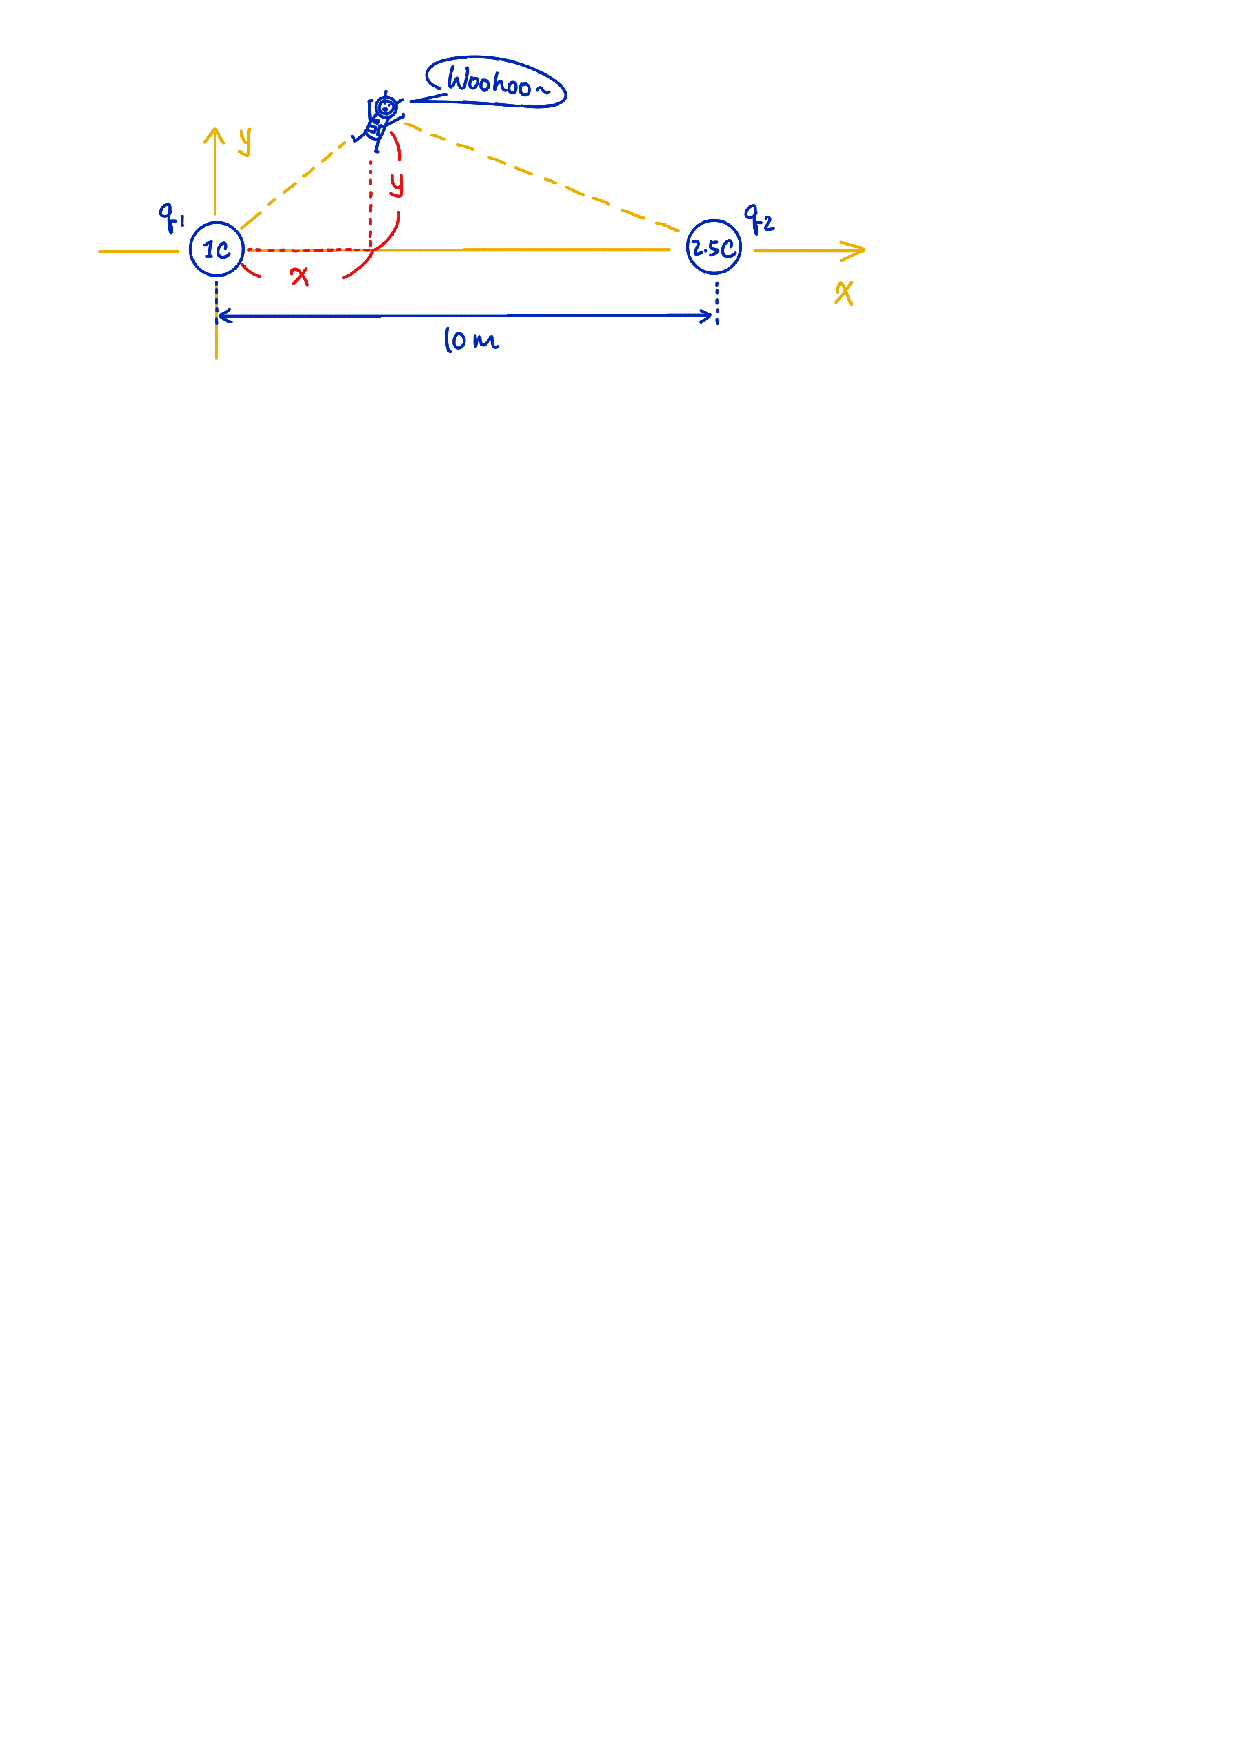
\includegraphics[scale=0.8]{trianglePotential}
\end{center}
\noindent Charge $q_2=2.5\,$C is fixed at $\vec{x}_2 = (10 ,0)$\,m;\\
Charge $q_1 = 1\,$C is fixed at $\vec{x}_1 = (0,0)$\,m; \\ 
The Coulomb constant $k = 8.99 \cdot 10^9$\,Nm$^2$/C$^2$, and the mass of an electron is $9.11 \cdot 10^{-31}\,$kg.\\

\noindent\textbf{Part\,(a)}: Draw a few equipotential lines around the two charges and in the region between the two charges. How do equipotential lines compare to electric field lines?\\
 
\noindent\textbf{Part\,(b)}: Find the electric potential in this configuration at a point $\vec{x}=(x,y)$ ``between" the two charges. That is, you can assume $0<x<10$ meters, but allow an arbitrary value for $y$. \\


\begin{center}
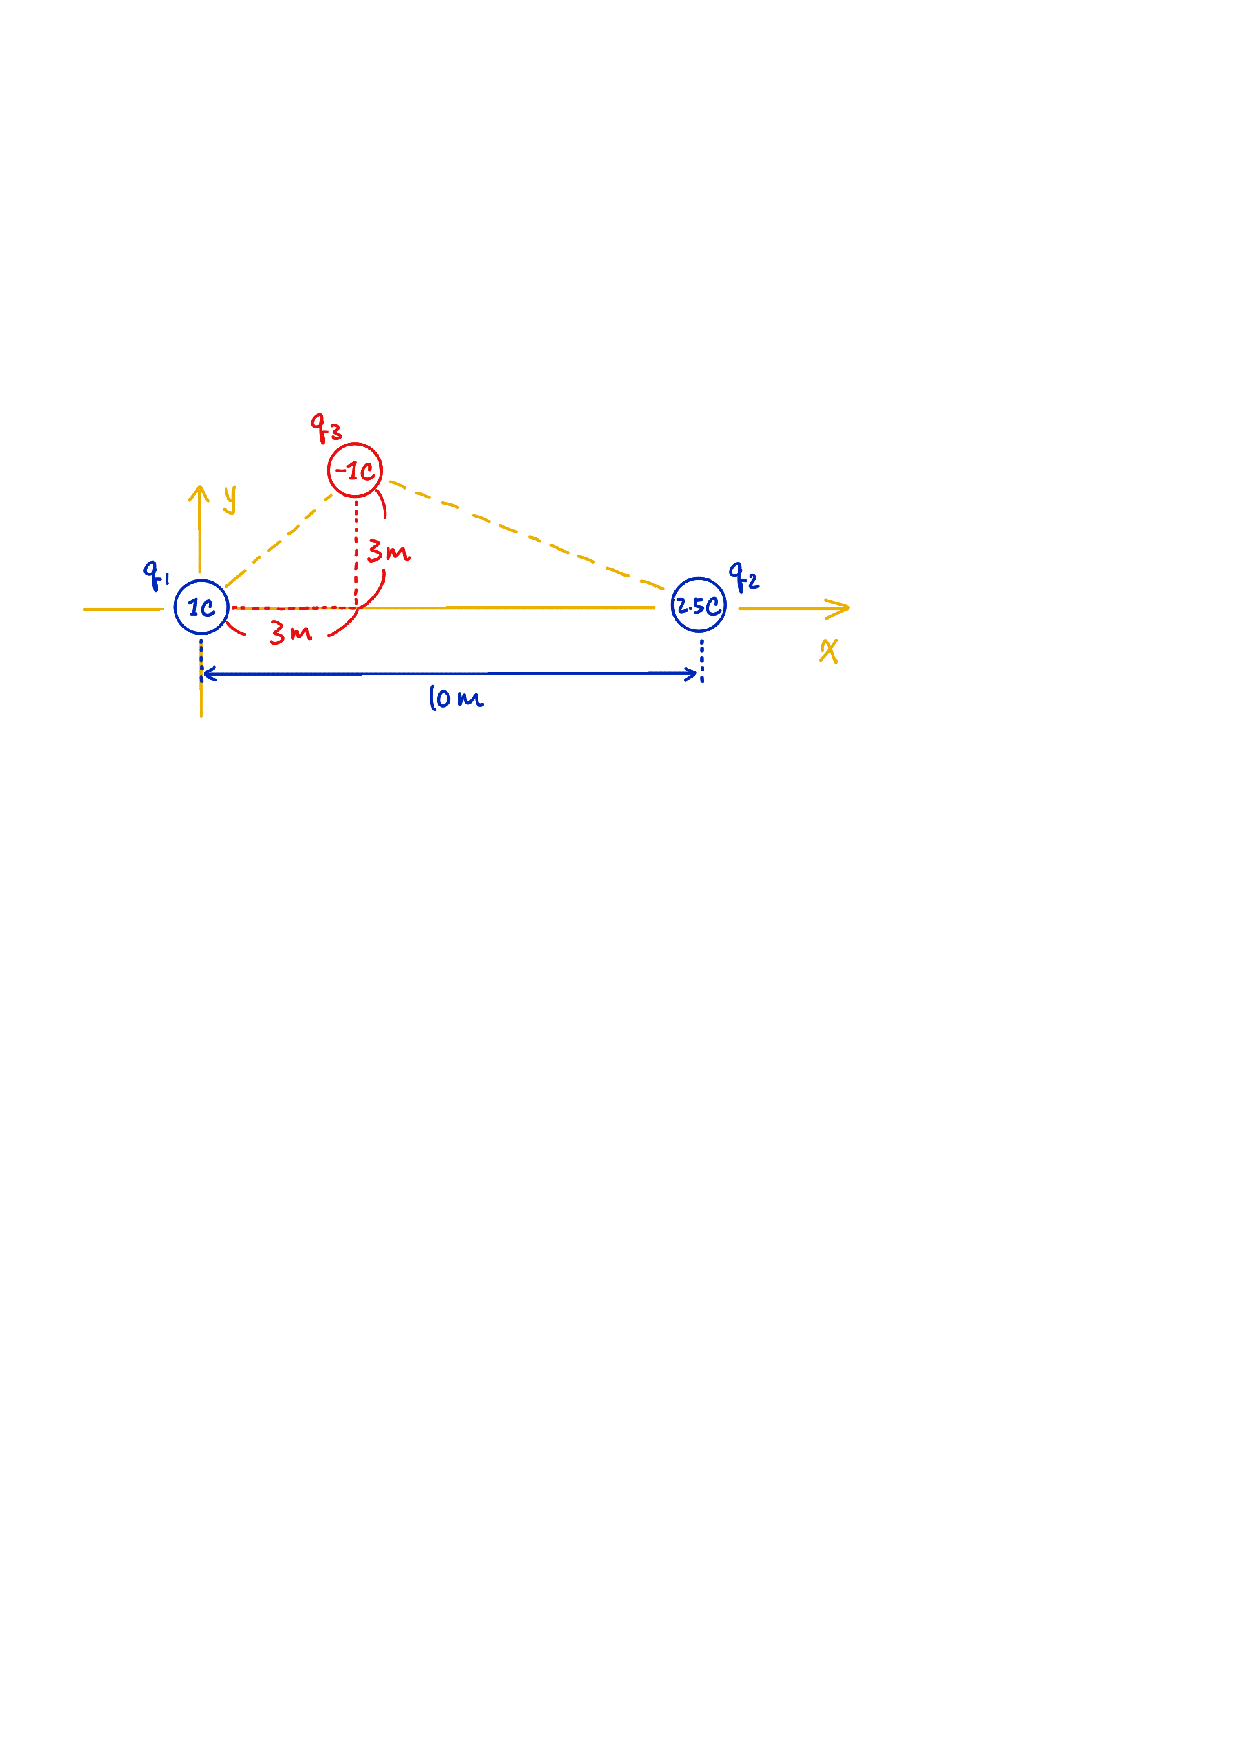
\includegraphics[scale=0.8]{trianglePE}
\end{center}
\noindent Now we place another charge $q_3=-1$\,C at $\vec{x}_i = (3,3)$\,m. \\

\noindent\textbf{Part\,(c)}: Find the amount of work needed to move $q_3$ from $\vec{x}_i = (3,3)$ to $\vec{x}_f = (3,0)$\,m.\\

\noindent\textbf{Part\,(d)}: Find the amount of work needed to move $q_3$ from $\vec{x}_i = (3,3)$ to $\vec{x}_f = (3,-3)$\,m.\\

\newpage
\noindent\textbf{Problem 2}: [The computation in this problem should be very very easy.]\\
Suppose in a $2$-dimensional region we have an electric potential $V(x) = x+10$ (with units of volts). That is, the electric potential depends only on the $x$-coordinate of the location, and does not depend on the $y$-coordinate. \footnote{The unit for $x$ is meter. If the unit for $V(x) = \alpha x+\beta$ is V, then the unit for the constant $\alpha$ is V/m and the unit for the constant $\beta$ is V. Therefore, in this problem, $\alpha=1$\,V/m and $\beta = 10\,$V.}\\

\noindent\textbf{Part (a)}: Draw in the coordinate system a few equipotential lines, and label their potential. Then draw the electric field lines based on the equipotential lines.\\

\begin{center}
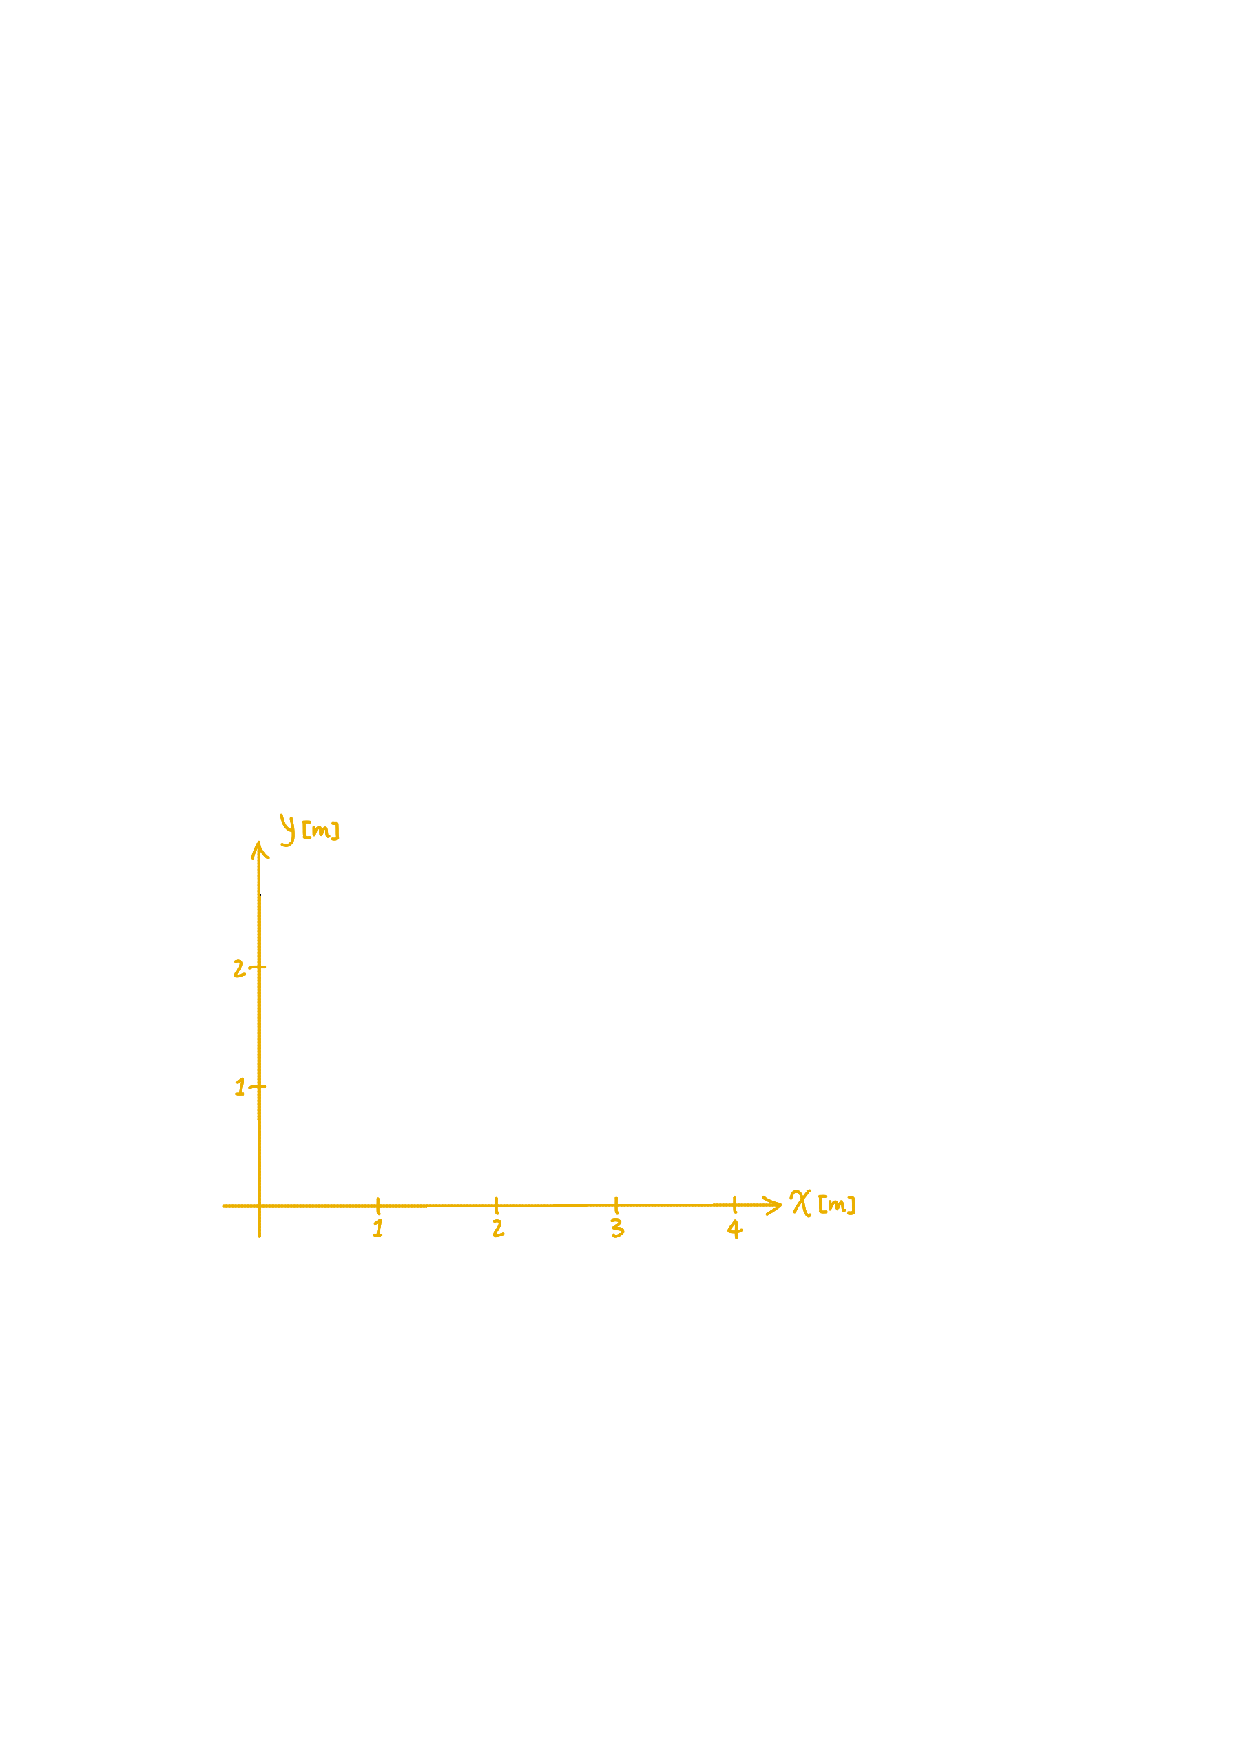
\includegraphics[scale=0.8]{gauge}
\end{center}

\noindent\textbf{Part (b)}: Find the electric field in its vector form $\vec{E} = (E_x,\, E_y)$ at $\vec{x}_1 = (1,0)$\,m.\\

\noindent\textbf{Part (c)}: Find the electric field in its vector form $\vec{E} = (E_x,\, E_y)$ at $\vec{x}_2 = (3,3)$\,m.\\

\noindent\textbf{Part (d)}: If the electric potential is $V(x) = x + 233333$ instead, find the electric field at position $\vec{x}_1=(1,0)$\,m and at position $\vec{x}_2 = (3,3)\,$m.\\



\newpage
\section*{Problem 1}
It is unclear how we can draw the equipotential lines in this configuration, but we know the relation between electric field lines and equipotential lines - electric field lines are always perpendicular to the equipotential lines - so we can use this fact to draw the equipotential lines.
\begin{center}

\includegraphics[scale=0.8]{mountains}
\end{center}
\noindent Notice at all points where the blue lines (electric field lines) intersect with the red lines (equipotential lines), the two are perpendicular to each other. The blue lines on the right are denser than the blue lines on the left, and this is because the charge on the right is ``larger" than the charge on the left. The equipotential lines form a ``contour map," like the top view of two mountains, with the one on the right slightly larger than the one on the left.\\

At a point $\vec{x}$ between the two charges, we can first find the electric potential $V_1$ at $\vec{x}$ due to $q_1$ on the left, then find the electric potential $V_2$ at $\vec{x}$ due to $q_2$ on the right, and sum the two to get the total potential at $\vec{x}$. Here $V_1$ is first computed, 
\begin{align*}
V_1 = \frac{kq_1}{r_1}\,,
\end{align*}
where $r_1 = \sqrt{(x-0)^2 + (y-0)^2} = \sqrt{x^2+y^2}$ is the distance between the point $\vec{x}$ and the charge $q_1$ located at the origin. Therefore, we can write
\begin{align*}
V_1 = \frac{kq_1}{\sqrt{x^2 + y^2}}\,.
\end{align*}
\textbf{Caution: Electric potential is a scalar, so it does not have $x$- or $y$-component. There is no $\sin$ or $\cos$ that you need to consider here}. Similarly, for $V_2$, we have
\begin{align*}
V_2 = \frac{kq_2}{r_2}\,,
\end{align*}
where $r_2 = \sqrt{(10-x)^2 + (y-0)^2} = \sqrt{(10-x)^2 + y^2}$ is the distance between the point $\vec{x}$ and the charge $q_2$ located at $(10,0)$\,m. Therefore, summing the two, we have
\begin{align*}
V = V_1 + V_2 = \frac{kq_1}{\sqrt{x^2+y^2}}+ \frac{kq_2}{\sqrt{(10-x)^2+y^2}}=
\frac{8.99 \cdot 10^9}{\sqrt{x^2+y^2}}+ \frac{22.48 \cdot 10^9}{\sqrt{(10-x)^2+y^2}}\,.
\end{align*}
The unit for $V$ is Volt.\\

Now if I put another charge $q_3$ into this region, from week-3 discussion worksheet, we know that $q_3$ will have electric potential energy 
\begin{align*}
U = q_3V = (-1)\cdot \left(\frac{8.99 \cdot 10^9}{\sqrt{x^2+y^2}}+ \frac{22.48 \cdot 10^9}{\sqrt{(10-x)^2+y^2}}\right)\,. \tag{*}
\end{align*}
I need to plug in $x = 3$ and $y=3$ to evaluate this potential energy at position $\vec{x}_i = (3,3)\,$m, the place where $q_3$ is initially placed. Therefore, at $\vec{x}_i = (3,3)$\,m, 
\begin{align*}
U_i = -\frac{8.99 \cdot 10^9}{\sqrt{3^2+3^2}}-\frac{22.48 \cdot 10^9}{\sqrt{(10-3)^2+3^2}} = -5.07\cdot 10^9\, \text{J}
\end{align*}
Since I want to move $q_3$ to another position $\vec{x}_f = (3,0)$\,m, we also find the electric potential energy of $q_3$ at $\vec{x}_f = (3,0)$\,m using Eq.\,(*). 
\begin{align*}
U_f = -\frac{8.99 \cdot 10^9}{\sqrt{3^2+0^2}}-\frac{22.48 \cdot 10^9}{\sqrt{(10-3)^2+0^2}} = -6.21 \cdot 10^9\,\text{J}\,.
\end{align*}
Due to energy conservation, 
\begin{align*}
\text{KE}_i+ U_i + (\text{External Work})= \text{KE}_f+ U_f\,,
\end{align*}
with initial and final kinetic energy being zero, the amount of energy that we need to spend to move $q_3$ from the initial position $\vec{x}_i$ to the final position $\vec{x}_f$, which is exactly the ``external" work done to $q_3$, is just the potential energy difference at the two points. That is, 
\begin{align*}
\text{External Work} = U_f - U_i = -6.21 \cdot 10^9 - (-5.07\cdot 10^9) = -1.14\cdot 10^9\,\text{J}\,.
\end{align*}
This is the final answer for part (c). The reason that we need to spend negative work to move $q_3$ from the initial position to the final position is because the electric force acting on $q_3$ (due to $q_1$ and $q_2$) at $\vec{x}_i = (3,3)\,$m is already helping us to pull $q_3$ down towards $\vec{x}_f = (3,0)$\,m. We only need to prevent $q_3$ from moving further down when it reaches  $\vec{x}_f = (3,0)$\,m, so we only need to apply a force upwards on $q_3$ to stop its motion, and that force is anti-aligned with the displacement of the charge (moving downwards). Since 
\begin{align*}
W = \vec{F}\cdot \Delta \vec{x}\,,
\end{align*} 
if $\vec{F}$ points in a direction opposite to $\Delta \vec{x}$, the work $W$ is negative.\\

Now we repeat our calculation for moving $q_3$ from $\vec{x}_i= (3,3)$\,m to $\vec{x}_f = (3,-3)$\,m. At the final position $\vec{x}_f = (3,-3)$\,m, using Eq.\,(*) again, we have 
\begin{align*}
U_f = -\frac{8.99 \cdot 10^9}{\sqrt{3^2+(-3)^2}}-\frac{22.48 \cdot 10^9}{\sqrt{(10-3)^2+(-3)^2}} = -5.07\cdot 10^9\, \text{J}\,.
\end{align*}
We notice that $U_i$ is exactly the same as $U_f$ (with $U_i$ computed above at $\vec{x}_i = (3,3)\,$m). Therefore, we conclude that 
\begin{align*}
\text{External Work} = U_f - U_i =0\,\text{J}\,.
\end{align*} 
This indicates that $\vec{x}_i=(3,3)$\,m and $\vec{x}_f = (3,-3)\,$m are on the same equipotential line, as they have the same potential due to $q_1$ and $q_2$, such that $q_3$ has the same electric potential energy at the two points. \textbf{It is a fact that, if friction is neglected, it takes zero work for moving a test charge from one point on an equipotential line to another point on the same equipotential line.} There is another point of view that we can understand this: It takes a negative amount of work $W_1$ to move $q_3$ from $(3,3)\,$m to $(3,0)$\,m because the electric force on $q_3$ is helping us, but it takes positive amount of work $W_2$ to move $q_3$ from $(3,0)$\,m to $(3,-3)\,$m because the electric force on $q_3$ is no longer helping us. In fact, from $(3,0)$\,m to $(3,-3)$\,m, the electric force is ``counter-helping" us. You can verify that the electric force is trying to pull $q_3$ upwards when $q_3$ travels from $(3,0)$\,m to $(3,-3)$\,m. Therefore, in the entire process, we have $W_1 +W_2 = 0$, the positive and the negative works cancel exactly. \\

\section*{Problem 2}
Again, as in Problem 1, the electric field lines should be perpendicular to the equipotential lines. Along each equipotential line, we have the same electric potential. Since $V(x)$ depends only on $x$, the equipotential lines are vertical straight lines in the region. Therefore, the electric field lines are straight lines in the horizontal direction, pointing from large potential to small potential (because positive charge creates positive electric potential while negative charges create negative electric potential). 
\begin{center}

\includegraphics[scale=0.8]{grid}
\end{center}

To find the electric field from the given potential $V(x) = x+10$, we need to use the relation 
\begin{align*}
E_x = -\frac{\Delta V}{\Delta x}\,,\qquad
E_y = -\frac{\Delta V}{\Delta y}\,. \tag{$\dagger$}
\end{align*} 
The ``$\Delta$" means the change in something. The calculus version of this statement is
\begin{align*}
\vec{E} = -\nabla V = \left( -\frac{\partial V}{\partial x}\,,\ -\frac{\partial V}{\partial y}\right)\,.
\end{align*}
But I am not allowed to talk about calculus in this class so ... Let us stick with the non-calculus version, but then there is one key thing you need to know about the equations ($\dagger$): \textbf{The statement $E_x = -\Delta V / \Delta x$ applies only to uniform electric field $E_x$ and electric potential $V$ that linearly depends on $x$,} such as the one we have in this problem. Here ``uniform" means that the quantity is the same everywhere in space.\\

First we want to find $E_x$, let's say we have $\Delta x = 1$ meter, then the change in $V(x)$ under the $1$-meter change in $x$ is $1$ Volt, and this is true regardless of where we measure such a change. That is, near $\vec{x} = (1,0)$\,m,  if we go from $x_i = 0.5$\,m to $x_f = 1.5$\,m, we see that $V(x)$ changes from $0.5+10 = 10.5$\,Volts to $1.5+10 = 11.5$\,Volts. Similarly, near $\vec{x} = (3,3)$\,m,  if we go from $x_i =2.5$\,m to $x_f = 3.5$\,m, we see that $V(x)$ changes from $2.5+10 = 12.5$\,Volts to $3.5+10 = 13.5$\,Volts. In both cases, $V(x)$ increases by $1$ volt. Now we conclude
\begin{align*}
E_x = -\frac{\Delta V}{\Delta x} = -1\,\text{V/m}\,.
\end{align*}
You can use the similar argument to find that 
\begin{align*}
E_y = -\frac{\Delta V}{\Delta y} = 0 \,\text{V/m}\,,
\end{align*}
but a more straightforward way to see this is from the fact that $V(x)$ does not depend on the $y$-position, so no matter how much you change your $y$-coordinate, the corresponding $\Delta V$ is zero, hence $E_y = 0$\,V/m. This answers part (b) and (c) together, 
\begin{align*}
\vec{E} = (-1,0)\,\text{V/m}
\end{align*}
at either $\vec{x}_1 = (1,0)$\,m or $\vec{x}_2 = (3,3)\,$m, as we just argued that such a unit change in $V$ does not depend on where we measure it. In fact, the quantity $\Delta V/\Delta x$ is the slope of the line $V(x)$, and therefore, $\vec{E}$ is sort of the negative ``slope" of $V$ (in higher-dimensional space, this is called the negative gradient of $V$). Also due to this, we see that only the coefficient in front of $x$ in $V(x)$ matters, the $+10$ in $V(x)=x+10$ does not matter at all. There is a special name for that constant term ``$+10$" in Physics: It is called the gauge in $V(x)$. The statement is that changing the gauge in $V(x)$ does not change the electric field $\vec{E}$ at all. \\


In the argument above, we see that the constant term ``$+10$" in the original $V(x)$ does not matter, so the electric fields at $\vec{x}_1$ and $\vec{x}_2$, even if we change to $V(x)= x+ 233333$, stay the same as before,
\begin{align*}
\vec{E} = (-1,\,0)\,\text{V/m}\,.
\end{align*}
This corresponds to a statement that you have learned in Physics 5A: The value of energy does not matter, only the energy difference between two points in space matters. That is, the statement here is that the \textbf{value of electric potential does not matter, but the electric potential difference at two different points does matter}, and we have used this exact statement in our calculation of Problem 1 Parts (c) and (d). 

\begin{center}
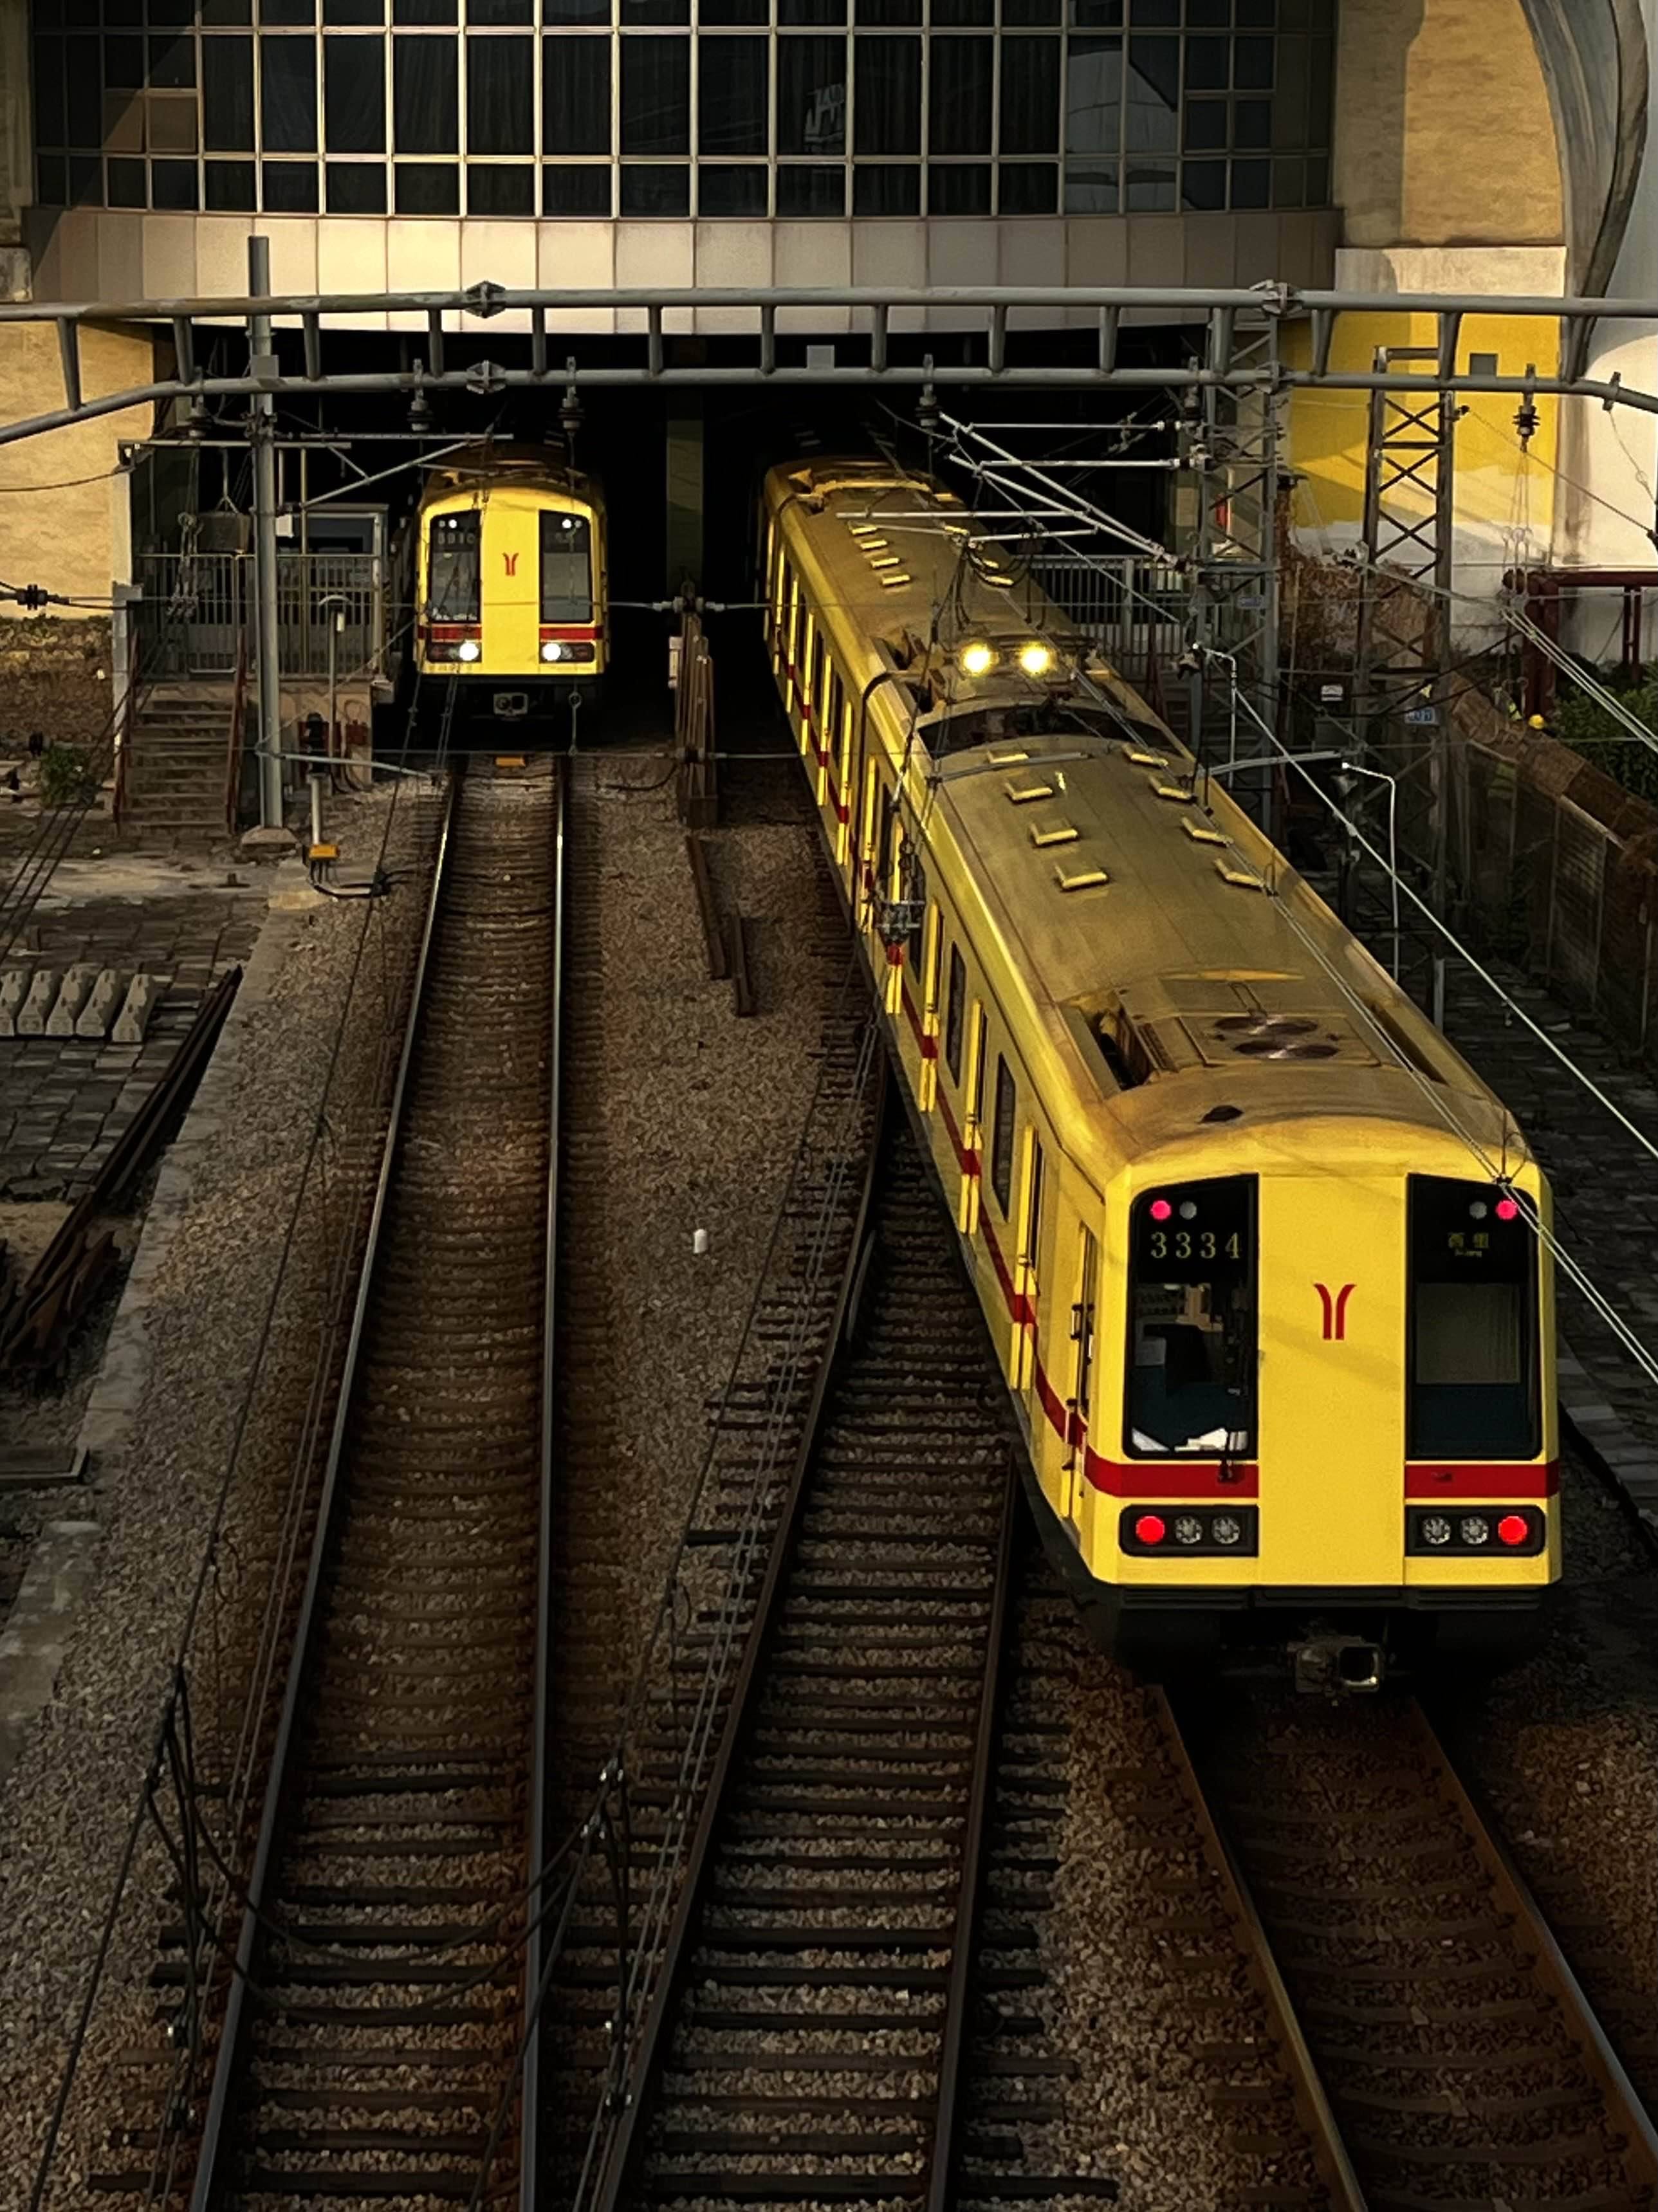
\includegraphics[scale=0.15]{line1}\\
\hfill\break
The photo of this week is metro lines in Guangzhou, China.\ \ \ :D
\end{center}




\end{document}


